\section{Arquitectura de LINUX}

	Tomando en cuenta el libro Operating Systems-Internals and Description de William Stallings, responda lo siguiente:

	\begin{itemize}

		\item ¿Cuál es la arquitectura de LINUX?
		\\La mayoría de los kernels de Unix son monolíticos. Si se realizan cambios en cualquier parte de un sistema operativo típico monolítico, todos los módulos y rutinas deben ser reinstalados y vueltos a vincular y el sistema debe ser rebooteado para que los cambios surtan efecto. Este problema es especialmente agudo para Linux, por lo cual el desarrollo es global y realizado por un grupo estrechamente asociado de programadores independientes.
Aunque Linux no utiliza un enfoque microkernel, logra muchas de las ventajas potenciales de este enfoque a través de su particular \textbf{arquitectura modular}. \\

		\item ¿Qué se entiende por loadable modules?
		\\Linux está estructurado como un conjunto de módulos, un número de las cuales puede cargarse y descargarse bajo demanda. Estos bloques relativamente independientes se denominan \textbf{loadable modules}.
En esencia, un módulo es un archivo objeto cuyo código puede ser vinculado y desvinculado del kernel en tiempo de ejecución. Típicamente, un módulo implementa una función específica, tal como un sistema de archivos, un controlador de dispositivo o alguna otra característica de la capa superior del núcleo.\\

		\item Mencione y describa las dos principales características que proporcionan el concepto de loadable modules:
		\\Los módulos cargables de Linux tienen dos características importantes:
\begin{enumerate}

	\item \textbf{Vinculación dinámica}: Un módulo del kernel puede ser cargado y enlazado en el kernel, mientras que el kernel ya está en la memoria y ejecutándose. Un módulo puede también ser desenlazado y eliminado de la memoria en cualquier momento.\\

	\item \textbf{Módulos apilables}: Los módulos están dispuestos en una jerarquía. Los módulos individuales sirven como bibliotecas cuando se hace referencia mediante los módulos de cliente más arriba en la jerarquía, y como clientes cuando hacen referencia a los módulos más abajo.\\
\end{enumerate}

		\item Muestre el diagrama de componentes de LINUX y descríbalos:
		\\En pocas palabras, los principales componentes del kernel son los siguientes:
\begin{enumerate}
\item \textbf{Señales}: El kernel utiliza señales para llamar a un proceso. Por ejemplo, las señales se utilizan para notificar a un proceso de ciertos defectos, tales como la división por cero.
\item \textbf{Llamadas al sistema}: La llamada al sistema es el medio por el cual un proceso solicita un servicio kernel específica. Hay varios cientos de llamadas al sistema, que puede ser más o menos agrupados en seis categorías: sistema de archivos, procesos, programación, comunicación entre procesos, sockets (redes) y diversos.
\item \textbf{Procesos y planificador}: Crea, gestiona y planifica los procesos.
\item \textbf{Memoria virtual}: Asigna y gestiona la memoria virtual para procesos.
\item \textbf{Sistemas de archivos}: Proporciona un espacio de nombres jerárquico global para archivos, directorios y otros objetos relacionados con archivos y proporciona las funciones del sistema de archivos.
\item \textbf{Protocolos de red}: Soporta la interfaz de sockets a los usuarios para el conjunto de protocolos TCP / IP.
\item \textbf{Controladores de dispositivo de caracteres}: Gestiona los dispositivos que requieren del kernel para enviar o recibir datos de un byte a la vez, como terminales, módems e impresoras.
\item \textbf{Controladores de dispositivos de bloque}: Gestiona los dispositivos que leen y escriben datos en bloques, como diversas formas de la memoria secundaria (discos magnéticos, CD-ROM, etc.).
\item \textbf{Controladores de dispositivos de red}: Gestiona las tarjetas de interfaz de red y los puertos de comunicación que conectan a los dispositivos de red, tales como bridges y routers.
\item \textbf{Trampas y faltas}: Maneja las trampas y fallos generados por el procesador, tal como un fallo de memoria.
\item \textbf{Memoria física}: Gestiona el conjunto de marcos de página en la memoria real y asigna las páginas de memoria virtual.
\item \textbf{Interrupciones}: Maneja interrupciones desde los dispositivos periféricos.\\
\end{enumerate}
\centering
\begin{center}
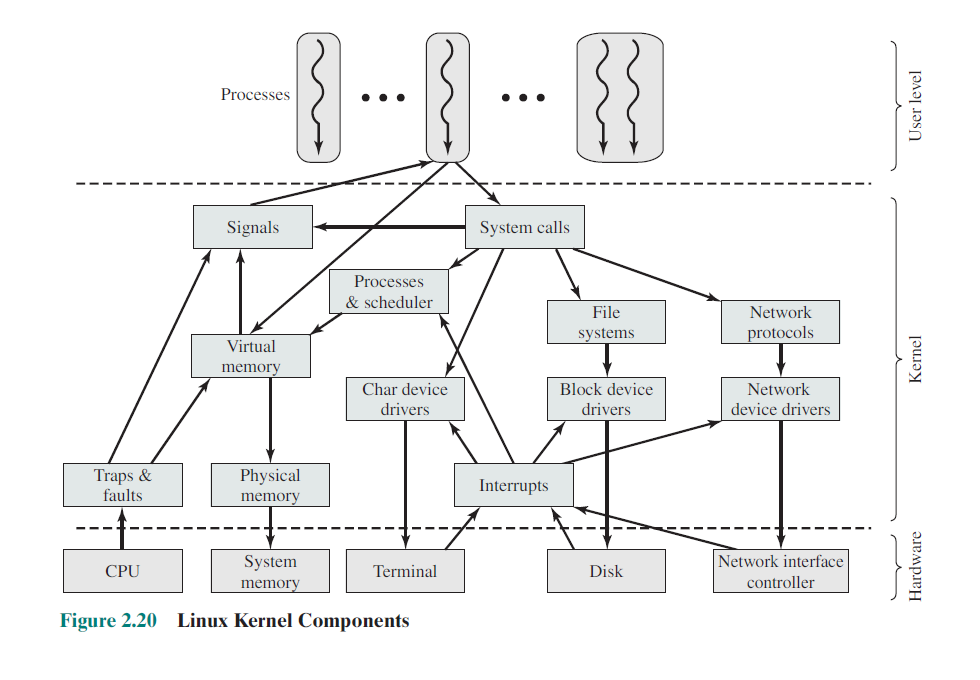
\includegraphics[width=\textwidth]{imagenes/componentes.png}
\end{center}

	\end{itemize}